\documentclass[ENG]{fancynotes}
\usepackage[utf8]{inputenc}
\usepackage[T1]{fontenc}
\usepackage[english]{babel}
\usepackage{amsmath, amssymb, amsfonts}
\usepackage{geometry}
\usepackage{graphicx}
\usepackage{hyperref}
\usepackage{float}
\usepackage{lmodern}
\usepackage{tikz}
\usetikzlibrary{arrows.meta, positioning, calc}
\usepackage{setspace}
\setlength{\parindent}{0pt}
\geometry{a4paper, left=2.0cm, right=2.0cm, top=2.0cm, bottom=2.0cm}
\setstretch{1.1}

\title{\vspace{2em}Derivation of the Normal Form for a Three-Alternative Decision Model\\ (Based on Roxin, 2019) }
\author{F. Javier Rodríguez Martínez}
\date{}

\begin{document}
\maketitle

\section{Model and Expansion}

We consider the following system for three alternatives:
\begin{align}
  \tau\,\dot{r}_L &= -r_L + \phi\Bigl(s_L\,r_L - c\,r_I + I_L + U\Bigr) +\xi_L(t) ,  \label{eq:rL}\\[1mm]
  \tau\,\dot{r}_C &= -r_C + \phi\Bigl(s_C\,r_C - c\,r_I + I_C + U\Bigr)+\xi_C(t), \label{eq:rC}\\[1mm]
  \tau\,\dot{r}_R &= -r_R + \phi\Bigl(s_R\,r_R - c\,r_I + I_R + U\Bigr)+\xi_R(t), \label{eq:rR}\\[1mm]
  \tau_I\,\dot{r}_I &= -r_I + \phi_I\Bigl(\frac{g}{3}\bigl(r_L+r_R+r_C\bigr)+I_I\Bigr)+\xi_I(t). \label{eq:rI}
\end{align}

In a summarized form:

\begin{align}
  \tau\,\dot{r}_i &= -r_i + \phi\Bigl(s_i\,r_i - c\,r_I + I_i + U\Bigr)+\xi_i(t), \quad i=L,C,R, \label{eq:exc}\\[1mm]
  \tau_I\,\dot{r}_I &= -r_I + \phi_I\Bigl(\frac{g}{3}(R_L+R_C+R_R)+I_I\Bigr)+\xi_I(t), \label{eq:inh}
\end{align}
where:
\begin{itemize}
  \item \(r_i\) is the firing rate of excitatory population \(i\).
  \item \(r_I\) is the firing rate of the inhibitory population.
  \item \(s_i\) is the self-excitation coefficient (which may differ among populations).
  \item \(c\) is the inhibition coefficient.
  \item \(I_i\) are each population external input.
  \item \(U\) is a ramping urgency signal. We assume it varies slowly:
    \[
    U = U_0 + \varepsilon^2\,\Delta U.
    \]
	As U is a ramping signal, we have that $U_0 = 0$
  \item \(\tau\) and \(\tau_I\) are the time constants for the excitatory and inhibitory populations, respectively.
\end{itemize}

Our goal is to derive a reduced (normal form) model that captures the critical dynamics in a two-dimensional competitive subspace.

An schematic representation of the model is shown in figure \ref{fig:model-rates}.

\begin{figure}[H]
\centering
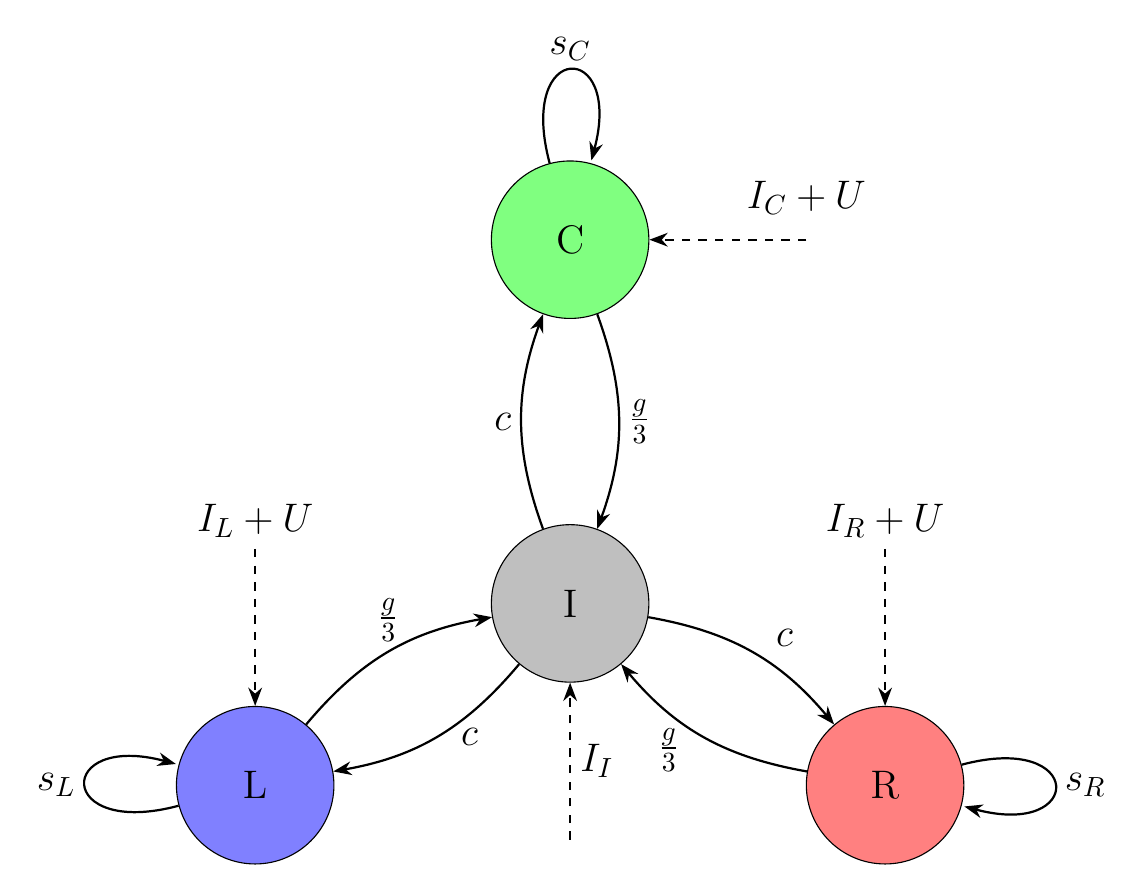
\begin{tikzpicture}[>=Stealth,
  neuron/.style={draw, circle, minimum size=2.0cm, inner sep=4pt, font=\Large},
  arrowlabel/.style={draw=none, fill=none, font=\Large}]

  % Define positions for the excitatory neurons (L, C, R)
  % For an equilateral triangle of side 8:
  % L at (-4, 0), R at (4, 0), C at (0, 6.928)
  \node[neuron, fill=blue!50] (L) at (-4,0) {L};
  \node[neuron, fill=green!50] (C) at (0,6.928) {C};
  \node[neuron, fill=red!50] (R) at (4,0) {R};
  
  % The inhibitory neuron (I) is placed at the centroid:
  % Centroid of triangle with vertices (-4,0), (4,0), (0,6.928) is at (0, (0+0+6.928)/3) = (0,2.309)
  \node[neuron, fill=gray!50] (I) at (0,2.309) {I};

  % Draw self-loops (representing self-excitation) for each excitatory neuron.
  \draw[->, thick] (L) edge[loop left] node[arrowlabel, left] {$s_L$} (L);
  \draw[->, thick] (C) edge[loop above] node[arrowlabel, above] {$s_C$} (C);
  \draw[->, thick] (R) edge[loop right] node[arrowlabel, right] {$s_R$} (R);

  % Draw connections from each excitatory neuron to the inhibitory neuron.
  \draw[->, thick, bend left=20] (L) edge node[arrowlabel, above] {$\tfrac{g}{3}$} (I);
  \draw[->, thick, bend left=20] (C) edge node[arrowlabel, right] {$\tfrac{g}{3}$} (I);
  \draw[->, thick, bend left=20] (R) edge node[arrowlabel, left, xshift = -5pt, yshift = -5pt] {$\tfrac{g}{3}$} (I);

  % Draw feedback connections from the inhibitory neuron to each excitatory neuron.
  \draw[->, thick, bend left=20] (I) edge node[arrowlabel, right, xshift = 5pt] {$c$} (L);
  \draw[->, thick, bend left=20] (I) edge node[arrowlabel, left] {$c$} (C);
  \draw[->, thick, bend left=20] (I) edge node[arrowlabel, right, xshift = 5pt, yshift = 5pt] {$c$} (R);

  % Draw external input arrows (dashed) to each excitatory neuron.
  \draw[->, dashed, thick] ($(L)+(0,3)$) -- (L) node[arrowlabel, pos = 0, yshift = 10pt ] {$I_L+U$};
  \draw[->, dashed, thick] ($(C)+(3,0)$) -- (C) node[arrowlabel, pos = 0, yshift = 15pt] {$I_C+U$};
  \draw[->, dashed, thick] ($(R)+(0,3)$) -- (R) node[arrowlabel, pos = 0, yshift = 10pt ]  {$I_R+U$};
  % Draw external input arrow to the inhibitory neuron.
  \draw[->, dashed, thick] ($(I)+(0,-3)$) -- (I) node[arrowlabel, midway, right] {$I_I$};

\end{tikzpicture}
\caption{Schematic representation of the rate model for 3-choice tasks. The choices are represented by three excitatory populations labeled L (Left), C (Center), and R (Right), which receive external inputs ($I_L$, $I_C$, and $I_R$, respectively) and exhibit self-excitation with strengths $s_L$, $s_C$, and $s_R$. There's also an external ramping input U common to all the excitatory populations. Each excitatory population affects to an inhibitory population (I) with weight $g/3$, and the inhibitory neuron provides feedback with strength $c$ to all excitatory populations. An external input $I_I$ is also applied to the inhibitory neuron.}
\label{fig:model-rates}
\end{figure}
\newpage


\subsection{Derivation of the normal form}

We assume a series expansion for the solution:
\begin{align}
  r_i(t) &= R_i + \varepsilon\,r_{1,i}(t) + \varepsilon^2\,r_{2,i}(t) + O(\varepsilon^3), \quad i=L,C,R, \label{eq:exp_ex}\\[1mm]
  r_I(t) &= R_I + \varepsilon\,r_{1,I}(t) + \varepsilon^2\,r_{2,I}(t) + O(\varepsilon^3). \label{eq:exp_inh}
\end{align}
The fixed point \(R=(R_1,R_2,R_3,R_I)\) is determined at \(O(1)\):
\begin{align}
  R_i &= \phi\Bigl(s_i\,R_i - c\,R_I + I_i \Bigr), \quad i=L,C,R, \label{eq:fixed_ex}\\[1mm]
  R_I &= \phi_I\Bigl(\frac{g}{3}(R_L+R_C+R_R)+I_I\Bigr). \label{eq:fixed_inh}
\end{align}

Additionally, we introduce a slow time scale:
\[
T = \varepsilon\,t,
\]
so that
\[
\frac{d}{dt} = \frac{\partial}{\partial t} + \varepsilon\,\frac{\partial}{\partial T}.
\]


We define
\begin{equation}
  X_i = s_i\,r_i - c\,r_I + I_i + U.
  \label{eq:argument}
\end{equation}
Substituting the expansions and using \(U =  \varepsilon^2\,\Delta U\), we have
\[
X_i = s_i\,(R_i + \varepsilon\,r_{1,i} + \cdots) - c\,(R_I + \varepsilon\,r_{1,I}+\cdots) + I_i + \varepsilon^2\,\Delta U.
\]
We then group:
\begin{itemize}
  \item Order \(O(1)\):
    \[
    X_{i,0} = s_i\,R_i - c\,R_I + I_i .
    \]
  \item Order \(O(\varepsilon)\):
    \[
    \delta X_i^{(1)} = \varepsilon\Bigl[s_i\,r_{1,i} - c\,r_{1,I}\Bigr].
    \]
  \item Order \(O(\varepsilon^2)\): includes the term \(\varepsilon^2\,\Delta U\).
\end{itemize}

The Taylor expansion of \(\phi\) about \(X_{i,0}\) is
\begin{equation}
  \phi(X_i) = \phi(X_{i,0}) + \phi'(X_{i,0})\,\delta X_i + \frac{1}{2}\,\phi''(X_{i,0})\,(\delta X_i)^2 + O(\varepsilon^3),
  \label{eq:taylor_exp}
\end{equation}
with
\[
\delta X_i = \varepsilon\Bigl[s_i\,r_{1,i} - c\,r_{1,I}\Bigr] + \varepsilon^2\,\Delta U.
\]
Thus,
\[
\phi\Bigl(s_i\,r_i - c\,r_I + I_i + U\Bigr) = \phi(X_{i,0}) + \varepsilon\,\phi'(X_{i,0})\Bigl(s_i\,r_{1,i} - c\,r_{1,I}\Bigr) + \varepsilon^2\left(\phi'(X_{i,0})\,\Delta U + \frac{1}{2}\,\phi''(X_{i,0})\Bigl(s_i\,r_{1,i} - c\,r_{1,I}\Bigr)^2\right) + O(\varepsilon^3).
\]


For the equation (\ref{eq:exc}), substituting the expansion we have:

At \(O(1)\):
\[
R_i = \phi(X_{i,0}), \quad i=L,C,R.
\]
At \(O(\varepsilon)\):
\begin{align}
  \tau\,\frac{d}{dt}\Bigl(R_i + \varepsilon\,r_{1,i}\Bigr) &= -\Bigl(R_i + \varepsilon\,r_{1,i}\Bigr) \nonumber\\[1mm]
  &\quad + \phi(X_{i,0}) + \varepsilon\,\phi'(X_{i,0})\Bigl[s_i\,r_{1,i}-c\,r_{1,I}\Bigr] + O(\varepsilon^2).
  \label{eq:order1}
\end{align}
Since \(R_i=\phi(X_{i,0})\), the \(O(1)\) terms cancel. Thus, dividing by \(\varepsilon\) we obtain:
\begin{equation}
  \tau\,\dot{r}_{1,i} = \Bigl[-1 + s_i\,\phi'(X_{i,0})\Bigr] r_{1,i} - c\,\phi'(X_{i,0})\,r_{1,I}, \quad i=L,C,R.
  \label{eq:order1_excitatory}
\end{equation}
The \textbf{bifurcation condition} we impose is:
\begin{equation}
  s_i\,\phi'(X_{i,0}) = 1, \quad i=L,C,R.
  \label{eq:bifurcation_condition}
\end{equation}
Under this condition, (\ref{eq:order1_excitatory}) reduces to:
\begin{equation}
  \tau\,\dot{r}_{1,i} = - c\,\phi'(X_{i,0})\,r_{1,I}, \quad i=L,C,R.
  \label{eq:order1_ex_final}
\end{equation}

Similarly, linearizing the inhibitory equation (\ref{eq:inh}) gives:
\begin{equation}
  \tau_I\,\dot{r}_{1,I} = -r_{1,I} + \phi_I'\Bigl(\frac{g}{3}(R_L+R_C+R_R)+I_I\Bigr)\frac{g}{3}\,\sum_{i=L,C,R}r_{1,i}.
  \label{eq:order1_inhibitory}
\end{equation}

Then the $O(\epsilon)$ equations can be written as
\[
L_0\,r_1 = 0,
\]
with
\begin{frame}
\footnotesize
\setlength{\arraycolsep}{2.5pt} % default: 5pt
\medmuskip = 1mu % default: 4mu plus 2mu minus 4mu
\[ 
  L_0 = \begin{pmatrix}
    0 & 0 & 0 & c\,\phi'(X_{L,0}) \\[2mm]
    0 & 0 & 0 & c\,\phi'(X_{C,0}) \\[2mm]
    0 & 0 & 0 & c\,\phi'(X_{R,0}) \\[2mm]
    -\dfrac{g}{3}\,\phi_I'\Bigl(\frac{g}{3}(R_L+R_C+R_R)+I_I\Bigr) & -\dfrac{g}{3}\,\phi_I'\Bigl(\frac{g}{3}(R_L+R_C+R_R)+I_I\Bigr) & -\dfrac{g}{3}\,\phi_I'\Bigl(\frac{g}{3}(R_L+R_C+R_R)+I_I\Bigr) & 1
  \end{pmatrix}.
  \label{eq:L0_matrix}
\]
\end{frame}
Here, \(X_{i,0} = s_i\,R_i - c\,R_I + I_i\). 
\bigskip
\bigskip

Due to the slow time scale \(T=\varepsilon\,t\), the time derivative expands as:
\[
\frac{d}{dt} = \frac{\partial}{\partial t} + \varepsilon\,\frac{\partial}{\partial T}.
\]
The contribution from the slow scale (when acting on \(r_1\)) appears at order \(\varepsilon^2\) and is grouped into the operator \(L_1\):
\begin{equation}
  L_1 = \begin{pmatrix}
    \tau\,\partial_T & 0 & 0 & 0 \\[2mm]
    0 & \tau\,\partial_T & 0 & 0 \\[2mm]
    0 & 0 & \tau\,\partial_T & 0 \\[2mm]
    0 & 0 & 0 & \tau_I\,\partial_T
  \end{pmatrix}.
  \label{eq:L1_matrix}
\end{equation}

\bigskip
At order \(\varepsilon^2\), we collect terms from the Taylor expansion (\ref{eq:taylor_exp}). Recall that
\[
\delta X_i = \varepsilon\Bigl[s_i\,r_{1,i}-c\,r_{1,I}\Bigr] + \varepsilon^2\,\Delta U.
\]
Thus, from (\ref{eq:taylor_exp}) we have:
\begin{equation}
  \phi(X_i) = \phi(X_{i,0}) + \varepsilon\,\phi'(X_{i,0})\Bigl(s_i\,r_{1,i}-c\,r_{1,I}\Bigr) + \varepsilon^2\left(\phi'(X_{i,0})\,\Delta U + \frac{1}{2}\,\phi''(X_{i,0})\Bigl(s_i\,r_{1,i}-c\,r_{1,I}\Bigr)^2\right) + O(\varepsilon^3).
  \label{eq:taylor_full2}
\end{equation}
If the inputs have the form
\[
I_i = I_0 + \varepsilon^2\,\bar{I}_i,
\]
then the order \(\varepsilon^2\) term for the \(i\)th excitatory equation is:
\begin{equation}
  N_{2,i} = \phi'(X_{i,0})\Bigl(\bar{I}_i + \Delta U\Bigr) + \frac{1}{2}\,\phi''(X_{i,0})\Bigl[s_i\,r_{1,i}-c\,r_{1,I}\Bigr]^2.
  \label{eq:N2_excitatory}
\end{equation}
An analogous term \(N_{2,I}\) is obtained for the inhibitory equation from the expansion of \(\phi_I\).

Thus, the order \(\varepsilon^2\) equation is written as
\begin{equation}
  L_0\,r_2 + L_1\,r_1 = N_2,
  \label{eq:order2_eq}
\end{equation}


Since \(L_0\) has a nontrivial null space (by the bifurcation condition), a solution for \(r_2\) exists only if the forcing term \(N_2 - L_1\,r_1\) is orthogonal to the null space of the adjoint of \(L_0\). Let \(\{e_1,e_2\}\) be a basis for this null space, for example, we choose:
\[
e_1 = (1, -1, 0, 0), \quad e_1 = (1, 1, -2, 0).
\]
The \textbf{solvability condition} is given by:
\begin{equation}
  \langle e_j,\; L_1\,r_1 - N_2 \rangle = 0,\quad j=1,2.
  \label{eq:solvability_cond}
\end{equation}
Expressing the first-order solution in the form
\[
r_1 = e_1\,X_1(T) + e_2\,X_2(T),
\]
Where $X_1 = r_L-r_C, X_2 =  r_L+r_C-2r_R, $

The normal form equations are:
\begin{align}
  \tau\,\dot{X}_1 &= A_1\,\bigl(\bar{I}_L - \bar{I}_C\bigr) + A_1\,\Delta U + C_1\,X_1\,X_2 + A_1 (\xi_L(t)-\xi_C(t)) + O(\epsilon^3), \label{eq:normal_form1}\\[2mm]
  \tau\,\dot{X}_2 &= A_2\,\bigl(\bar{I}_L + \bar{I}_C - 2\bar{I}_R\bigr) + A_2\,\Delta U + C_2\,\bigl(X_1^2 - 3X_2^2\bigr) +  A_2(\xi_L(t)+\xi_C(t)-2\xi_R(t)) + O(\epsilon^3). \label{eq:normal_form2}
\end{align}

Here, the coefficients are given in terms of the initial parameters as follows:
\[
\begin{aligned}
A_1 &= \frac{1}{2}\Bigl[\phi'(X_{L,0}) - \phi'(X_{C,0})\Bigr], \quad
& A_2 &= \frac{1}{6}\Bigl[\phi'(X_{L,0}) + \phi'(X_{C,0}) - 2\,\phi'(X_{R,0})\Bigr],\\[1mm]
C_1 &= \frac{1}{2}\Bigl[s_L^2\,\phi''(X_{L,0}) - s_C^2\,\phi''(X_{C,0})\Bigr], \quad
& C_2 &= \frac{1}{6}\Bigl[s_L^2\,\phi''(X_{L,0}) + s_C^2\,\phi''(X_{C,0}) - 2\,s_R^2\,\phi''(X_{R,0})\Bigr].
\end{aligned}
\]

\bigskip
\noindent
% End of document



\end{document}
